\chapter{Theory and Background}
In this chapter, I will provide the theoretical background necessary to understand the work presented in this thesis. The first section will deal with the definition and importance of the bandgap of a material, the second will introduce the effects of confinement on electrons within semiconductors, leading to a useful physical model, the semiconductor quantum well. The third will introduce the concept of semiconductor quantum well disorder, and the fourth will motivate the study of semiconductor quantum well disorder with micro photoluminescence spectroscopy.

\section{The Semiconductor Quantum Well}
INTRO
\subsection{Bandgap}

%bandgap def, little discussion
\indent In order to understand the state of electrons in a crystalline solid, one must first understand how electrons act under the effect of a periodic potential. When we bring electron orbitals together in a molecule, the wave functions perturb each other. In the case of semiconductors, the Bloch theorem is a useful tool for understanding this problem quantum-mechanically, and a complete treatment can be found in CITE (Iadonisi and Siradesh). Fundamentally, if one assumes that valance electrons exist in an infinite, periodic, homogeneous lattice, then electron wave functions are invariant under translation from one lattice point to the next. The Bloch theorem state that under translation from lattice cite to lattice cite, the electron wavefunction will pick up a phase:

\begin{equation}
\vec{k}\cdot \vec{R_n}
\end{equation}
 
where $\vec{k}$ is the displacement wavevector and  $\vec{R_n}$ is the lattice vector for the $n$th lattice cite to which the wavefunction is translated CITE Iandonesi. Thus, the electron wavefunction becomes 
 \begin{equation}
 \psi(\vec{r}) = e^{i \vec{k\cdot r}} u_k(\vec{r})
 \end{equation}
where $\vec{r}$ is the lattice coordinate and $u_k(\vec{r})$ is a periodic function for each primitive cell in the crystal. In the limit that many primitive cells are brought together in a crystal, two things happen: each n-fold degenerate electronic energy level will split into n components, and these levels will become so close that they will smear into allowed and disallowed energy bands CITE Indonesi, Siradesh, Grif, Davies. If electrons have a high enough energy, they can occupy the `conduction band' states where they are free to move about the lattice structure. They are otherwise confined to their host atoms and occupy the `valance band' states. The energy difference between the valance band and conduction band is called the bandgap, and is illustrated in the example dispersion curve, \ref{Example band structure of a direct-gap semiconductor.}. 

\begin{figure}[h!]
\centering
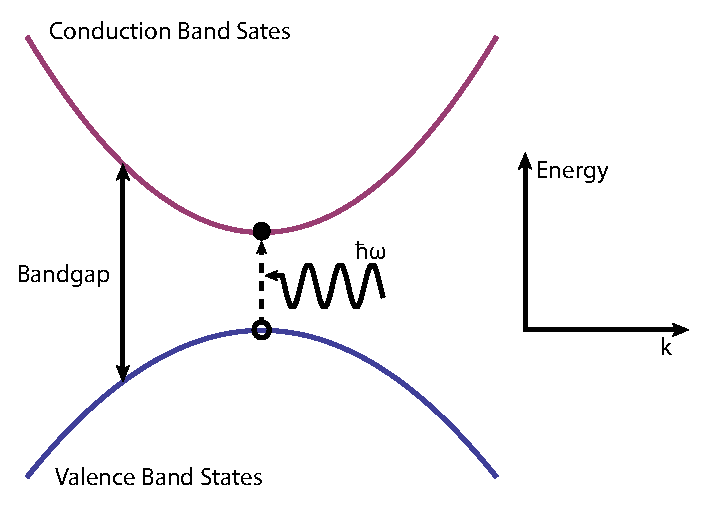
\includegraphics[width = .7\textwidth]{dispcurve.eps}
\caption{A typical dispersion curve minima for a direct-gap semiconductor. An optical transition is illustrated at $\vec{k} = 0$, where an electron is emitting a photon as the result of a transition from the conduction band to the valance band.}
\label{ExampleBands}
\end{figure}

%dispersion curves
\indent The full functional shape of dispersion curves is dependent on the physical properties of solids. Thus, solids can be broadly construed into three categories: metals, insulators, and semiconductors. In metals, the conduction band energies are below the Fermi level and thus some electrons are free to move about and conduct charge. In insulators, the bandgap is relatively large, and therefore electrons are confined to their host atoms. By contrast in semiconductors, the bandgap is fairly small and therefore only a small amount of energy is required to promote an electron to the conduction band from the valance band. Importantly, semiconductor electrons can be photo-excited into the conduction band CITE Iandonesi. This fact forms the basis of experimental studies of semiconductor nanostructures (CITE Steve review), photonic devices, and certain types of theoretical quantum information processing schemes (CITE Nature Review of QI).

%Discussion of bands in GaAs and AlGaAs, p orbital smearing etc. Find p 63 in davies.
(Discussion of band structure in GaAs arising from p-orbital smearing, figure highlighting the direct-gap nature of GaAs).

\subsection{Confinement and The Exciton}
%confinement intro
\indent It is well known that nanometer scale confinement of particles results in quantized energy states CITE Griff. In the previous section, I briefly introduced the bandgap, and its important physical properties. In this section, I'll illustrate an interesting application of band theory: the semiconductor quantum well. First, it is important to understand what we mean by confinement, and how quantized energy levels arise for confined particles. I will then construct a physical picture of the semiconductor quantum well (QW), and then I will discuss the formation of excitons and a simple physical model of their behavior, sufficient for understanding the spectroscopy conducted in this thesis.

\indent Perhaps the simplest problem in quantum mechanics is the of confinement of a particle in a finite, one dimensional potential well. I will sketch a derivation of the wave function of a particle trapped in such a well, and use this derivation as the basis for exploring the physics of the QW exciton. We will begin by considering an arbitrary particle confined in a one dimensional infinite potential well. The potential that our arbitrary particle feels is:

\[ V(x) = \begin{cases} 
      0 & 0 < x < L \\
      \infty & |x| > 0 
   \end{cases}
\]
where $L$ is the length of the potential well. Graphically, the potential the particle feels looks like \ref{infp}.

\begin{figure}[h!]
\centering
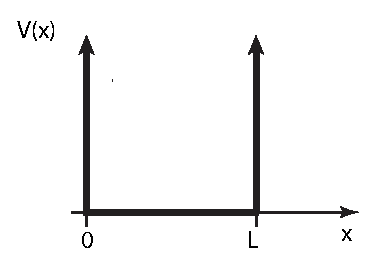
\includegraphics[width = .6\textwidth]{infpotential.eps}
\caption{A graphical representation of the one-dimensional infinite potential well of width $L$.}
\label{infp}
\end{figure}
Our task is to solve the time independent Schr\"{o}dinger equation to show how quantized bound states arise for one-dimensional confinement. The time independent Schr\"{o}dinger equation reads:

\begin{equation}
\hat{H} \psi = E\psi
\end{equation}
where E is the energy of the particle, and $\ket{psi}$ is the particle's wavefunction. The particle will evidently be confined to the well, so our Hamiltonian inside the well is just

\begin{equation}
\hat{H} = - \frac{\hbar^2}{2m} \frac{\partial^2}{\partial x^2}
\label{hamil}
\end{equation}
where $m$ is the particle's mass, and $E$ is the particle's total energy. The time independent Schr\"{o}dinger equation now reads:

\begin{equation} \label{tise}
\frac{\partial^2}{\partial x^2} \psi = - \alpha \psi
\end{equation}

where we define 

\begin{equation}
\alpha = \frac{2mE}{\hbar^2}.
\end{equation}
Now, eq. 2.4 looks like the familiar simple harmonic oscillator equation from classical mechanics. Because the wave function must be continuous at $x = L$ and $ x = 0$, i.e. it vanishes at those locations, and the potential is odd about the origin,  solutions to eq. 2.5 have the form:

\begin{equation} \label{soln1}
\psi(x) = A sin(k x) 
\end{equation}

where $k$ contains $E$ and is determined by our boundary conditions. Now we want $\psi(L)$ to vanish, but we can't have $A =0$, because that is the trivial solution to eq. 2.5. Therefore, because we want $\psi(L) = Asin(k L) = 0 $, we must have $ka = \pm n \pi$ where $n \in \mathbb{N}$. Now, we can absorb all of the negative combinations of $k L$ into our normalization constant, $A$. We have, then, that 

\begin{equation}
k_n L = n \pi 
\end{equation}

where the subscript denotes the fact that we now have infinitely many, \textit{discreet} solutions to eq. 2.5. Evidently 

\begin{equation}
k_n = \frac{ n \pi}{L}
\end{equation}

and therefore

\begin{equation}
\psi(x) = A sin(\frac{n \pi x}{L}).
\end{equation}

Now, if we let $k_n = \alpha$ and solve for E, we obtain

\begin{equation}
E = \frac{n^2 \pi^2 \hbar^2}{2 m L^2}.
\end{equation}
It will do us no good to normailze the wavefunctions we found, as I am not interested in the exact behavior of each state for our particle. The important part is that confinement in one dimension resulted in our particle occupying \textit{discreet} energy levels. 

\indent Using layers of semiconductors, one can generate similar confinement of electrons in one dimension. A simple way of confining particles is to sandwich a low-bandgap semiconductor in between two layers of higher bandgap materials (CITE Davies). One period of this structure is shown in figure \ref{}. If the well material is a direct-gap semiconductor, then simple vertical optical transitions across the bandgap can be made, as the transition illustrated in \ref{Example band structure of a direct-gap semiconductor.}. Figure \ref{GaAsBstruct} is the band structure for GaAs, the chosen well material for the studies of growth disorder. Annotated on the figure is the direct-gap transition zone of interest. The potential well created by the semiconductor sandwich leads to quantization of electron states within the well layer CITE Miller, Davies, Steve Review. We can access these transitions optically, making the QW a great testbed for exploring electron dynamics within a simple and well-known potential CITE Steve Review. 

\begin{figure}[h!]
\centering
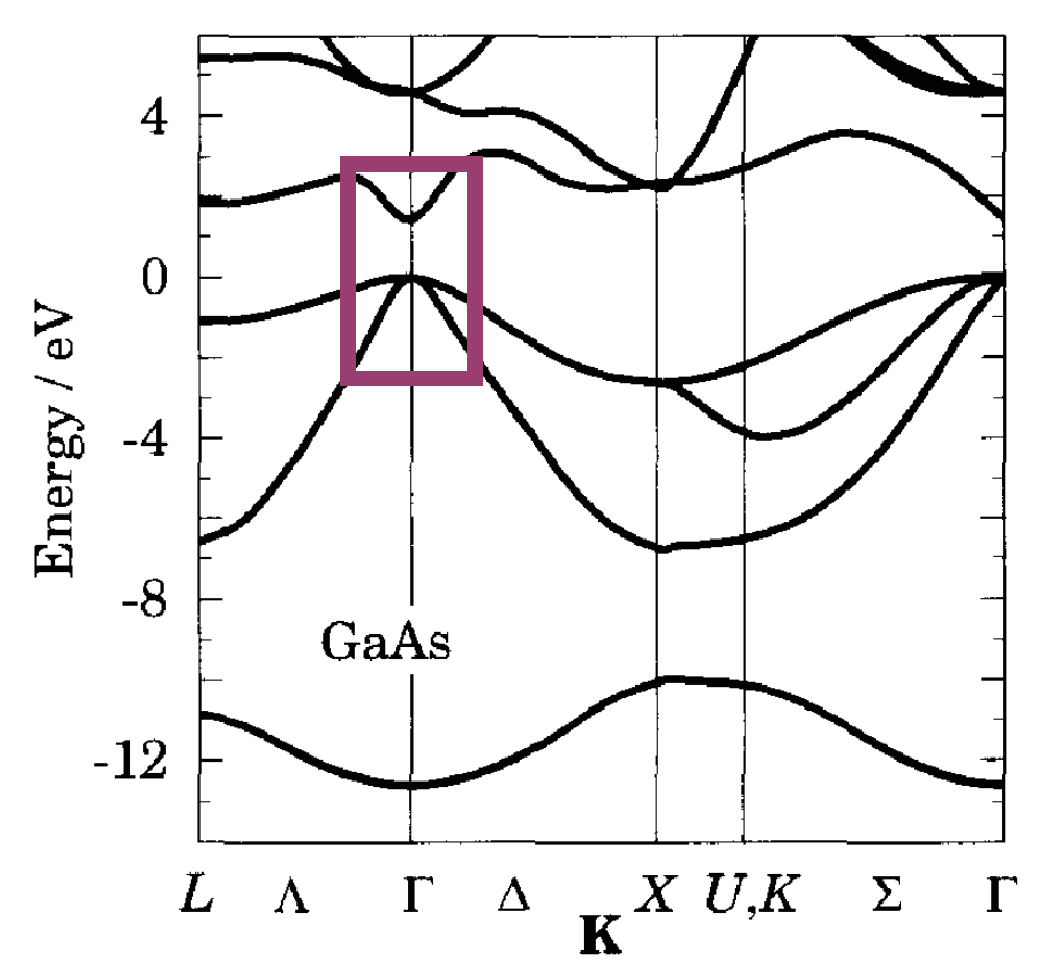
\includegraphics[width = .5\textwidth]{GaAsBstruct.eps}
\caption{The band structure of GaAs, the allowed states are the thick horizontal curves, and the boxed region is the direct-gap region, in which electrons can be photo-excited across the gap. Note, the minima of this region look like the dispersion curve in \ref{GaAsBstruct}.}
\label{GaAsBstruct}
\end{figure}


\begin{figure}[h!]
\centering
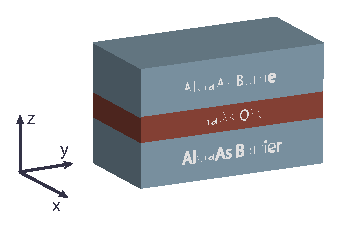
\includegraphics[width = .5\textwidth]{Well.eps}
\caption{An example of the semiconductor quantum well. These layers can be repeated arbitrarily many times with arbitrary dimension and thickness for many types of application.}
\label{GaAsBstruct}
\end{figure}




\indent The simple picture presented above doesn't quite adequately represent the physics of an electron within a quantum well, however. After an excited electron moves from the valence band to the conduction band, it will leave behind a vacancy, or `hole', around its parent atom CITE Miller, Davies. The electron feels a \textit{screened Coulomb potential} from this vacancy, as the vacancy is positively charged. I'll briefly sketch why this potential arises and then introduce the key concept of this section: the excition. Imagine a large number of electrons have been excited to their first excited state within the quantum well. Now, spatially, one will have a quasi-neutral distribution of electrons and holes in the well layer. Imagine inserting into this situation a positive charge. Adjacent electrons will immediately surround the positive charge, modifying the total Coulomb potential due to that charge, \textit{screening} its effects from charges far away. This phenomenon, known as Debye shielding CITE Chen, modifies the potential electrons feel from adjacent holes. If the potential electrons feel was exactly Coulombic in nature, then any bound state between an electron and a hole would be Hydrogenic CITE Griffiths. This potential, however, is \textit{not} exactly Culombic in nature, so the bound states between the electrons and holes don't exhibit exactly Hydrogenic behavior. The subtleties of the functional form of the wave function are treated in CITE Rogers, but a sketch of their form is in figure \ref{}. The photoexcited electron and an hole can form a bound pair, known as an exciton. The energy levels of this quasiparticle are discretized by its confinement in the quantum well. Additionally, coherent coupling of exciton states can be explored using multidimensional coherent spectroscopy CITE Steve Review, Bristow's PRL. 


\section{Quantum Well Disorder}






\section{Microphotoluminescence Spectroscopy}

\section{Asymmetric Double Quantum Wells}
\section{Photoluminescence Excitation Spectroscopy}